\section{Experimental Process}

\subsection{Data Analysis and Preprocessing}
In order to obtain valuable models for predicting hospital readmission, I need to perform a series of data analysis and preprocessing steps. These steps are crucial to ensure that the data are clean, well-structured, and suitable for machine learning algorithms.
\subsubsection{Overview of the Dataset}
The dataset used in this analysis comprises 101,766 individual observations, where each observation corresponds to a unique hospital encounter for a patient. It contains a total of 48 features, which can be logically grouped into several categories based on their nature and relevance to the analysis.\\
Firstly, the \textbf{demographic features} capture essential patient characteristics, such as race, gender, age, and weight. These variables provide a foundational understanding of the patient population and can be useful for identifying disparities or trends across different groups.\\
The second group consists of \textbf{hospitalization details}, which describe the circumstances and duration of the hospital stay. These include variables like the type of admission, discharge disposition, admission source, and the length of stay in days. Such features are critical for understanding the context of each hospital encounter and may also reflect the severity or urgency of the patient's condition.\\
Next, the dataset includes \textbf{administrative information}, which refers to aspects related to the healthcare provider and organization.\\
A particularly informative group is the \textbf{healthcare utilization} features, which quantify how intensively healthcare resources were used during the patient's interaction with the system. This includes the number of lab tests performed, procedures conducted, medications administered, and counts of outpatient, emergency, and inpatient visits.\\
Another important category is the \textbf{diagnosis information}, which captures diagnostic codes assigned during the hospital encounter. These codes are essential for identifying the clinical conditions that led to hospitalization and can offer predictive insights into patient outcomes.\\
Additionally, the dataset includes \textbf{laboratory results}, which provide numerical values for specific tests such as blood glucose levels and other relevant biomarkers. These features allow for a more direct measurement of the patient's physiological state.\\
The \textbf{medication details} group is particularly extensive and offers a detailed look into the pharmacological treatment received by each patient. This includes information on specific medications prescribed or administered during the hospital stay.\\
Complementing this, there are also \textbf{general medication indicators}, which include two features: one indicating whether there was a change in diabetic medication and another reflecting whether diabetes medication was prescribed at all. These high-level indicators can reveal treatment decisions that may be associated with readmission risk.\\
Finally, the \textbf{target variable} captures whether or not a patient was readmitted to the hospital after discharge. In the original dataset, this information is categorized based on the time to readmission (e.g., within 30 days, after 30 days, or no readmission). For the purpose of this study, the target was simplified into a binary variable, distinguishing between patients who were readmitted and those who were not. Analyzing the distribution of this variable (as shown in Figure \ref{fig:target_distribution}) allows us to assess the class balance of the dataset, which is crucial for guiding the modeling strategy.\\




\begin{figure}[H]
    \centering
    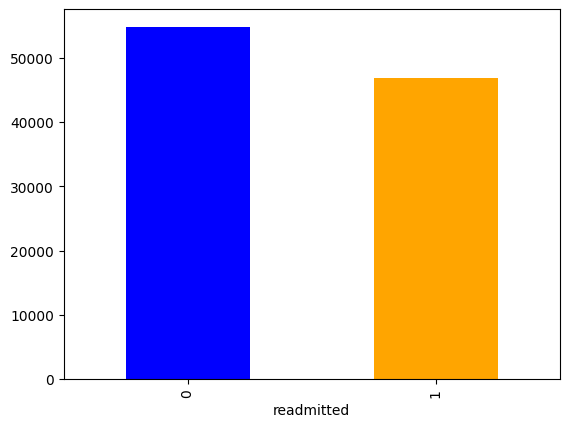
\includegraphics[width=0.8\textwidth]{images/balance.png}
    \caption{Distribution of the Target Variable}
    \label{fig:target_distribution}
\end{figure}

\subsubsection{Dealing with Missing Values}
After the initial Overview of the Dataset, we proceed to analyze and handle missing values. 
\begin{table}[H]
\centering
\caption{Percentage of Missing Values per Column}
\label{tab:missing-values}
\begin{tabular}{|l|c|}
\hline
\textbf{Column} & \textbf{Missing Values (\%)} \\
\hline
\texttt{race} & 2.23\% \\
\texttt{weight} & 96.86\% \\
\texttt{payer\_code} & 39.56\% \\
\texttt{medical\_specialty} & 49.08\% \\
\texttt{diag\_1} & 0.02\% \\
\texttt{diag\_2} & 0.35\% \\
\texttt{diag\_3} & 1.40\% \\
\texttt{max\_glu\_serum} & 94.75\% \\
\texttt{A1Cresult} & 83.28\% \\
\hline
\end{tabular}
\end{table}

\noindent
Columns such as \texttt{weight}, \texttt{max\_glu\_serum}, \texttt{A1Cresult}, \texttt{payer\_code}, and \texttt{medical\_specialty} present a high proportion of missing values, rendering them unsuitable for reliable analysis. As a result, these features are excluded from the dataset to preserve data integrity. For the remaining variables with lower levels of missingness, imputation is performed using the \textbf{mode}, taking into account the categorical nature and distributional characteristics of the data.

\subsubsection{Unique values and One-hot Encoding}
To prepare the dataset for machine learning models, it is essential to understand the categorical nature of various features. For this purpose, the number of unique values was computed for each categorical feature. Columns containing only a single unique value were subsequently removed, as they do not provide any discriminative information for the analysis.\\
After identifying the number of unique categories, I applied \textbf{One-Hot Encoding} to convert these categorical variables into a numerical format suitable for model training. This technique creates binary columns for each category, ensuring that the data is represented in a format that does not impose ordinal relationships among the categories, which is critical for preserving the integrity of nominal data.\\
As a result, the dataset is transformed into a format suitable for machine learning algorithms. The new shape of the dataset is (101766 rows × 103 columns), where the original 48 features have been expanded to 103 features due to the one-hot encoding of categorical variables.

\subsection{Creation of a Subset of the Original Dataset}
Considering the large size of the dataset, I created a subset to facilitate faster experimentation and model training. The subset is created by randomly selecting a portion of the original dataset, ensuring that it maintains the same distribution of the target variable.\\
The consequent subset contains 20353 observations and 103 features, which is a manageable size for initial model development and testing. 

\subsection{Data Splitting}
The dataset is split once into two parts, with the aim of creating a training set and a test set. The split is performed using a stratified approach to ensure that the distribution of the target variable is preserved in both sets.\\\\
The split is done as follows:
\begin{itemize}
    \item \textbf{Training set:} 80\% of the data
    \item \textbf{Test set:} 20\% of the data
\end{itemize}
\noindent
The training set is used for 5-fold cross-validation and hyperparameter tuning. Specifically, the training set is divided into 5 equal folds. In each of the 5 iterations, 4 folds are used for training the model, and 1 fold is used for validation. This ensures that every fold serves as the validation set exactly once, providing a robust evaluation of model performance during training.\\
The test set is held out and used only for the final evaluation of the model after cross-validation and tuning are complete.


\subsection{Evaluation Metrics}
To assess the performance of the machine learning models, several evaluation metrics are used: accuracy, F1 score, recall, and precision. Each of these metrics captures different aspects of model performance and provides a more complete understanding of how well the model is performing:
\begin{itemize}
    \item \textbf{Accuracy} In this case, that the dataset is not highly imbalanced, accuracy can be a useful metric as a general indicator of performance. 
    \item \textbf{Recall} (also known as sensitivity) evaluates the model’s ability to correctly identify positive cases. In the context of hospital readmission, this is crucial, as failing to detect patients who will be readmitted may have serious consequences.
    \item \textbf{Precision} High precision ensures that when the model predicts a readmission, it is likely to be correct, which is important to avoid unnecessary clinical interventions.
    \item \textbf{F1 Score} is the harmonic mean of precision and recall.
\end{itemize}
\noindent
Together, these metrics offer a comprehensive evaluation framework that goes beyond simple accuracy, helping to better understand the trade-offs and effectiveness of each model.

\subsection{Dimensionality Reduction through Feature Selection}

To reduce the dimensionality of the dataset and retain only the most informative features, we applied \textbf{Recursive Feature Elimination with Cross-Validation (RFECV)}. This method works by recursively removing the least important features based on the rankings produced by a specified estimator, while evaluating model performance at each iteration using cross-validation.
For this purpose, we selected a \textbf{Random Forest classifier} as the base estimator, owing to its robustness and its capability to provide meaningful feature importance scores. RFECV automatically determined the optimal number of features by maximizing the cross-validated \texttt{accuracy} score.
As a result, the original feature set was reduced from 103 to 30 features, retaining those most relevant for predicting hospital readmission. Subsequently, we applied the same procedures of hyperparameter tuning, cross-validation, and model evaluation described earlier, now using the reduced feature set.

\subsection{Hyperparameter Tuning, Cross-Validation, and test set evaluation}
I performed hyperparameter tuning using a grid search strategy. This approach systematically explores a predefined set of hyperparameter combinations to identify the configuration that yields the best performance.\\

\noindent Once the optimal hyperparameters were determined, I trained a new model using these settings and evaluated it using cross-validation. During cross-validation, performance metrics were computed for each fold, and the mean and standard deviation of each metric were calculated across all folds.\\

\noindent
Finally, to compare the models, I assessed their performance on the test set using the same evaluation metrics described previously, to see how well the models generalize to unseen data. 


\subsection{Machine Learning Models}
In order to remain consistent with the state of the art in predictive modeling, a heterogeneous set of machine learning models was selected. The goal was to explore different methodological paradigms, ranging from tree-based approaches to instance-based, probabilistic, and linear models. 

\paragraph{Decision Tree Classifier (DT).}
Decision Trees were chosen as an intuitive and interpretable baseline among tree-based methods. Their ability to handle both numerical and categorical attributes without requiring feature scaling makes them particularly robust for heterogeneous datasets such as the one considered.
\begin{tcolorbox}[colback=gray!5!white,colframe=gray!50!black,
                  boxrule=0.5pt,arc=2pt, left=1mm, right=1mm, top=0.5mm, bottom=0.5mm]
\texttt{criterion=gini, max\_depth=5, min\_samples\_split=2}
\end{tcolorbox}

\paragraph{Random Forest Classifier (RF).}
To extend the expressive power of a single decision tree, an ensemble of trees was constructed through Random Forests. 
\begin{tcolorbox}[colback=gray!5!white,colframe=gray!50!black,
                  boxrule=0.5pt,arc=2pt, left=1mm, right=1mm, top=0.5mm, bottom=0.5mm]
\texttt{criterion=gini, max\_depth=10, min\_samples\_split=5, n\_estimators=100}
\end{tcolorbox}

\paragraph{K-Nearest Neighbors (KNN).}
KNN was employed as a non-parametric, instance-based learning algorithm that makes no explicit assumptions about the data distribution. By relying on local neighborhood information, it provides a complementary decision-making perspective compared to tree ensembles and linear models. 
\begin{tcolorbox}[colback=gray!5!white,colframe=gray!50!black,
                  boxrule=0.5pt,arc=2pt, left=1mm, right=1mm, top=0.5mm, bottom=0.5mm]
\texttt{metric=manhattan, n\_neighbors=9, weights=uniform}
\end{tcolorbox}

\paragraph{Logistic Regression (LR).}
Logistic Regression was included as a linear and highly interpretable baseline. Despite its simplicity, it often performs competitively in high-dimensional settings and provides a clear probabilistic framework for binary classification. 
\begin{tcolorbox}[colback=gray!5!white,colframe=gray!50!black,
                  boxrule=0.5pt,arc=2pt, left=1mm, right=1mm, top=0.5mm, bottom=0.5mm]
\texttt{C=0.01, max\_iter=100, penalty=l1, solver=saga}
\end{tcolorbox}

\paragraph{Bernoulli Naive Bayes (BNB).}
Finally, Bernoulli Naive Bayes was selected for its computational efficiency and its suitability for binary-valued feature spaces, which align closely with the characteristics of several variables in the dataset. 
\begin{tcolorbox}[colback=gray!5!white,colframe=gray!50!black,
                  boxrule=0.5pt,arc=2pt, left=1mm, right=1mm, top=0.5mm, bottom=0.5mm]
\texttt{alpha=0.01, binarize=1.0, fit\_prior=True}
\end{tcolorbox}


